\setcounter{section}{4}
\section{ỨNG DỤNG ĐẠO HÀM VÀ KHẢO SÁT HÀM SỐ ĐỂ GIẢI QUYẾT MỘT SỐ BÀI TOÁN THỰC TIỄN}
\subsection{LÝ THUYẾT CẦN NHỚ}
\subsubsection{Tốc độ thay đổi của một đại lượng}
Ta có đạo hàm $f'(a)$ là tốc độ thay đổi tức thời của đại lượng $y=f(x)$ đối với $x$ tại điểm $x=a$. Dưới đây, chúng ta xem xét một số ứng dụng của ý tưởng này đối với vật lí, hoá học, sinh học và kinh tế: 
\begin{itemize}
	\item Nếu $s=s(t)$ là hàm vị trí của một vật chuyển động trên một đường thẳng thì $v=s'(t)$ biểu thị vận tốc tức thời của vật (tốc độ thay đổi của độ dịch chuyển theo thời gian). Tốc độ thay đổi tức thời của vận tốc theo thời gian là gia tốc tức thời của vật:
	$$
	a(t)=v'(t)=s''(t).
	$$
	\item Nếu $C=C(t)$ là nồng độ của một chất tham gia phản ứng hoá học tại thời điểm $t$, thì $C'(t)$ là tốc độ phản ứng tức thời (tức là độ thay đổi nồng độ) của chất đó tại thời điểm $t$.
	\item Nếu $P=P(t)$ là số lượng cá thể trong một quần thể động vật hoặc thực vật tại thời điểm $t$, thì $P'(t)$ biểu thị tốc độ tăng trưởng tức thời của quần thể tại thời điểm $t$.
	\item  Nếu $C=C(x)$ là hàm chi phí, tức là tổng chi phí khi sản xuất $x$ đơn vị hàng hoá, thì tốc độ thay đổi tức thời $C'(x)$ của chi phí đối với số lượng đơn vị hàng được sản xuất được gọi là chi phí biên.
	\item Về ý nghĩa kinh tế, chi phí biên $C'(x)$ xấp xỉ với chi phí để sản xuất thêm một đơn vị hàng hoá tiếp theo, tức là đơn vị hàng hoá thứ $x+1$ (xem SGK Toán 11 tập hai, trang 87, bộ sách Kết nối tri thức với cuộc sống). 
\end{itemize}
\subsubsection{Bài toán tối ưu hóa}
Một trong những ứng dụng phổ biến nhất của đạo hàm là cung cấp một phương pháp tổng quát, hiệu quả để giải những bài toán tối ưu hoá. Trong mục này, chúng ta sẽ giải quyết những vấn đề thường gặp như tối đa hoá diện tích, khối lượng, lợi nhuận, cũng như tối thiểu hoá khoảng cách, thời gian, chi phí.\\
Khi giải những bài toán như vậy, khó khăn lớn nhất thường là việc chuyển đổi bài toán thực tế cho bằng lời thành bài toán tối ưu hoá toán học bằng cách thiết lập một hàm số phù hợp mà ta cần tìm giá trị lớn nhất hoặc giá trị nhỏ nhất của nó, trên miền biến thiên phù hợp của biến số.\\
Quy trình giải một số bài toán tối ưu hoá  đơn giản:
\begin{itemize}
	\item[\iconCH]\indamm{Bước 1.} Xác định đại lượng Q mà ta cần làm cho giá trị của đại lượng ấy lớn nhất hoặc nhỏ nhất và biểu diễn nó qua các đại lượng khác trong bài toán.
	
	\item[\iconCH]\indamm{Bước 2.}  Chọn một đại lượng thích hợp nào đó, kí hiệu là $x$, và biểu diễn các đại lượng khác ở \indamm{Bước 1} theo $x$. Khi đó, đại lượng $Q$ sẽ là hàm số của một biến $x$. Tìm tập xác định của hàm số $Q=Q(x)$.
	
	\item[\iconCH]\indamm{Bước 3.}  Tìm giá trị lớn nhât hoặc giá trị nhỏ nhất của hàm số $Q=Q(x)$ bằng các phương pháp đã biết và kết luận.
\end{itemize}

\subsection{PHÂN LOẠI VÀ PHƯƠNG PHÁP GIẢI TOÁN}
\begin{dang}{Bài toán về tốc độ thay đổi của một đại lượng}
\end{dang}
\begin{vd}
	Khi bỏ qua sức cản của không khí, độ cao (mét) của một vật được phóng thẳng đứng lên trên từ điểm cách mặt đất $2$ m với vận tốc ban đầu $24{,}5$ m/s là $h(t)=2+24{,}5t-4{,}9t^2$ (theo Vật lí đại cương, NXB Giáo dục Việt Nam, $2016$).
	\begin{enumerate}
		\item Tìm vận tốc của vật sau $2$ giây.
		\item Khi nào vật đạt độ cao lớn nhất và độ cao lớn nhất đó là bao nhiêu?
		\item Khi nào thì vật chạm đất và vận tốc của vật lúc chạm đất là bao nhiêu?
	\end{enumerate}
	\loigiai{
		\begin{enumerate}
			\item Theo ý nghĩa cơ học của đạo hàm, vận tốc của vật là $v=h'(t)=24{,}5-9{,}8t$ m/s.\\				
			Do đó, vận tốc của vật sau $2$ giây là $v(2)=24{,}5-9{,}8\cdot 2=4{,}9$ m/s.
			\item Vì $h(t)$ là hàm số bậc hai có hệ số $a=-4{,}9< 0$ nên $h(t)$ đạt giá trị lớn nhất tại $t=-\dfrac{b}{2a}=\dfrac{24{,}5}{2\cdot 4{,}9}=2{,}5$ (giây). Khi đó, độ cao lớn nhất của vật là $h(2{,}5)=32{,}625$ m.
			\item Vật chạm đất khi độ cao bằng 0, tức là $h=2+24{,}5t-4{,}9t^2=0$, hay $t \approx 5{,}08$ (giây).\\
			Vận tốc của vật lúc chạm đất là $v(5{,}08)=24{,}5-9{,}8\cdot 5{,}08=-25{,}284$ m/s.\\
			Vận tốc âm chứng tỏ chiều chuyển động của vật là ngược chiều dương (hướng lên trên) của trục đã chọn (khi lập phương trình chuyển động của vật).
		\end{enumerate}
	}
\end{vd}

\begin{vd}
	Xét phản ứng hóa học tạo ra chất $C$ từ hai chất $A$ và $B$: $A+B\longrightarrow C$. Giả sử nồng độ của hai chất $A$ và $B$ bằng nhau $[A]=[B]=a$ (mol/l). Khi đó, nồng độ của chất $C$ theo thời gian $t$ ($t>0$) được cho bởi công thức: $[C]=\dfrac{a^2Kt}{aKt+1}$ (mol/l), trong đó $K$ là hằng số dương.
	\begin{enumerate}
		\item Tìm tốc độ phản ứng ở thời điểm $t>0$.
		\item Chứng minh nếu $x=[C]$ thì $x'(t)=K(a-x)^2$.
		\item Nêu hiện tượng xảy ra với nồng độ các chất khi $t\longrightarrow +\infty$.
		\item Nêu hiện tượng xảy ra với tốc độ phản ứng khi $t\longrightarrow +\infty$.
	\end{enumerate}
	\loigiai{
		\begin{enumerate}
			\item Tìm tốc độ phản ứng ở thời điểm $t>0$.\\
			Tốc độ của phản ứng là đạo hàm của $[C]=\dfrac{a^2Kt}{aKt+1}$ theo biến $t$. Do đó 
			\[[C]^\prime =\left(\dfrac{a^2Kt}{aKt+1}\right)^\prime=\dfrac{a^2K\left(aKt+1\right)-a^2Kt\cdot aK}{\left(aKt+1\right)^2}=\dfrac{a^2K}{\left(aKt+1\right)^2}.\]
			\item Chứng minh nếu $x=[C]$ thì $x'(t)=K(a-x)^2$.\\
			Theo câu trên, nếu nếu $x=[C]$ thì $x^\prime(t)=\dfrac{a^2K}{\left(aKt+1\right)^2}$.\\
			Ta lại có 
			\[K(a-x)^2=K \left(a-\dfrac{a^2Kt}{aKt+1}\right)^2=\dfrac{a^2K}{\left(aKt+1\right)^2}.\]
			Vậy $x'(t)=K(a-x)^2$.
			\item Nêu hiện tượng xảy ra với nồng độ các chất khi $t\longrightarrow +\infty$.\\
			Ta có $\lim\limits_{t\to +\infty}[C]=\lim\limits_{t\to +\infty}\dfrac{a^2Kt}{aKt+1}=a\  (mol/l)$.\\
			Vậy nồng độ của chất $C$ dần đến $a\  (mol/l)$.
			\item Nêu hiện tượng xảy ra với tốc độ phản ứng khi $t\longrightarrow +\infty$.\\
			Ta có $\lim\limits_{t\to +\infty}x^\prime(t)=\lim\limits_{t\to +\infty}\dfrac{a^2K}{\left(aKt+1\right)^2}=0$.\\
			Vậy tốc độ  của phản ứng  dần đến $0$.\\
	\end{enumerate}}
\end{vd}

\begin{vd}
	Giả sử số lượng của một quần thể nấm men tại môi trường nuôi cấy trong phòng thí nghiệm được mô hình hoá bằng hàm số $P(t)=\dfrac{a}{b+\mathrm{e}^{-0{,}75t}}$, trong đó thời gian $t$ được tính bằng giờ. Tại thời điểm ban đầu $t=0$, quần thể có 20 tế bào và tăng với tốc độ $12$ tế bào/giờ. Tìm các giá trị của $a$ và $b$. Theo mô hình này, điều gì xảy ra với quần thể nấm men về lâu dài?
	\loigiai{
		Ta có $P'(t)=\dfrac{0,75a \mathrm{e}^{-0,75t}}{\left(b+\mathrm{e}^{-0{,}75t}\right)^2}, t \geq 0$.\\
		Theo đề bài, ta có $P(0)=20$ và $P'(0)=12$. Do đó, ta có hệ phương trình:
		$$
		\heva{&\dfrac{a}{b+1}=20 \\& \dfrac{0,75a}{(b+1)^2=12}} \Leftrightarrow \heva{&a=20(b+1)\\&\dfrac{15}{b+1}=12}
		$$
		Giải hệ phương trình này, ta được $a=25$ và $b=\dfrac{1}{4}$.\\
		Khi đó, $P'(t)=\dfrac{18{,}75\mathrm{e}^{-0{,}75t}}{\left(\dfrac{1}{4}+\mathrm{e}^{-0{,}75 t}\right)^2} > 0, \forall t \geq 0$, tức là số lượng quần thể nấm men luôn tăng.\\
		Tuy nhiên, do $\lim\limits_{t \rightarrow+\infty} P(t)=\lim\limits_{t \rightarrow+\infty} \dfrac{25}{\dfrac{1}{4}+\mathrm{e}^{-0{,}75t}}=100$ nên số lượng quần thể nấm men tăng nhưng không vượt quá $100$ tế bào. 
	}
\end{vd}

\begin{vd}
	Giả sử chi phí $C(x)$ (nghìn đồng) để sản xuất $x$ đơn vị của một loại hàng hoá nào đó được cho bởi hàm số $C(x)=30\,000+300x-2{,}5x^2+0{,}125x^3$.
	\begin{enumerate}
		\item Tìm hàm chi phí biên.
		\item Tìm $C'(200)$ và giải thích ý nghĩa.
		\item So sánh $C'(200)$ với chi phí sản xuất đơn vị hàng hoá thứ 201.
	\end{enumerate}
	\loigiai{
		\begin{enumerate}
			\item Hàm chi phí biên là $C'(x)=300-5x+0{,}375x^2$.
			\item Ta có $C'(200)=300-5\cdot 200+0,375\cdot 200^2=14300$.\\				
			Chi phí biên tại $x=200$ là $14\,300$ nghìn đồng, nghĩa là chi phí để sản xuất thêm một đơn vị hàng hoá tiếp theo (đơn vị hàng hoá thứ 201) là khoảng $14\,300$ nghìn đồng.
			\item Chi phí sản xuất đơn vị hàng hoá thứ $201$ là
			$$
			C(201)-C(200)=1\,004\,372{,}625- 990\,000=14\,372{,}625 \text { (nghìn đồng).}
			$$				
			Giá trị này xấp xỉ với chi phí biên $C'(200)$ đã tính ở câu b.
		\end{enumerate}
		
	}
\end{vd}

\begin{dang}{Bài toán tối ưu hoá đơn giản}
\end{dang}

\begin{vd}
	\immini{Một nhà sản xuất cần làm những hộp đựng hình trụ có thể tích $ 1 $ lít. Tìm các kích thước của hộp đựng để chi phi vật liệu dùng để sản xuất là nhỏ nhất (kết quả được tính theo centimét và làm tròn đến chứ số thập phân thứ hai).}{
	\begin{tikzpicture}[line join=round,line cap=round,line width=.6pt,font=\footnotesize,scale=0.45,>=stealth]
		\coordinate[label=right:$A$] (A) at (3,0);
		\coordinate[label=left:$O$] (O) at (0,0);
		\coordinate[label=right:$A'$] (A1) at ($(A)+(90:6)$);
		\coordinate[label=left:$O'$] (O1) at ($(O)+(90:6)$);
		\draw (A) arc (0:-180:3 and 3/4)--($(A1)!2!(O1)$) arc (180:0:3 and 3/4) arc (0:-180:3 and 3/4) (A)--(A1)--(O1);
		\draw[dashed] (O1)--(O)--(A) arc (0:180:3 and 3/4);
		\fill (O)circle(1.5pt) (O1)circle(1.5pt) (A)circle(1.5pt) (A1)circle(1.5pt);
\end{tikzpicture}}
	\loigiai{
		Đổi $1 \text{ lít} =1000 \text{ cm}^3$.
		\\
		Gọi $r( cm )$ là bán kính đáy của hình trụ, $h( cm )$ là chiều cao của hình trụ.
		\\
		Diện tích toàn phần của hinh trụ là $S=2 \pi r^2+2 \pi r h$.
		\\
		Do thể tích của hình trụ là $1000 \text{ cm}^3$ nên ta có: $1000=V=\pi r^2 h$, hay $h=\dfrac{1000}{\pi r^2}$.
		\\
		Do đó, diện tích toàn phần của hình trụ là $S=2 \pi r^2+\dfrac{2000}{r},\, r>0$.
		\\
		Ta cần tìm $r$ sao cho $S$ đạt giá trị nhỏ nhất. Ta có
		\begin{align*}
			&S'=4 \pi r-\dfrac{2000}{r^2}=\dfrac{4 \pi r^3-2000}{r^2};
			\\
			&S'=0 \Leftrightarrow \pi r^3=500 \Leftrightarrow r=\sqrt[3]{\dfrac{500}{\pi}}
		\end{align*}
		Bảng biến thiên
		\begin{center}
			
\begin{tikzpicture}[font=\footnotesize,thick,>=stealth]
				\tikzset{double style/.append style={double distance=1.5pt}}\tkzTabInit[nocadre=false,lgt=1.2,espcl=3.5,deltacl=0.6,lw=.75pt,color,colorL=green!50,colorV=green!50]
				{$r$ /1.2, $S'(r)$ /1, $S(r)$ /2.5}
				{$0$,$\sqrt[3]{\dfrac{500}{\pi}}$,$+\infty$}
				\tkzTabLine{ ,-,$0$,+, }
				\tkzTabVar{+/$+\infty$,-/$S\left( \sqrt[3]{\dfrac{500}{\pi}} \right)$,+/$+\infty$}
			\end{tikzpicture}
		\end{center}
		Khi đó
		$$
		h=\dfrac{1000}{\pi r^2}=\dfrac{1000}{\pi \sqrt[3]{\frac{250000}{\pi^2}}}=\dfrac{100}{\sqrt[3]{250 \pi}}.
		$$
		Vậy cần sản xuất các hộp đựng hình trụ có bán kinh đáy $r=\sqrt[3]{\dfrac{500}{\pi}} \approx 5,42 \text{ (cm)}$ và chiều cao $h=\dfrac{100}{\sqrt[3]{250 \pi}} \approx 10,84\text{ (cm)}$.
	}
\end{vd}

\begin{vd}
	Một bác nông dân có ba tấm lưới B40, mỗi tấm dài $a \text{ (m)}$ và muốn rào một mảnh vườn dọc bờ sông có dạng hình thang cân $ABCD$ như {\it Hình 36} (bờ sông là đường thẳng $CD$ không phải rào). Hỏi bác đó có thể rào được mảnh vườn có diện tích lớn nhất là bao nhiêu mét vuông?
	\begin{center}
		\begin{tikzpicture}[scale=.6]
			\path 
			(-3,0) coordinate (D)
			(3,0) coordinate (C)
			($(D)+(65:3)$) coordinate (A)
			($(C)+(115:3)$) coordinate (B)
			;
			\fill[cyan!50] (-4.5,-1) rectangle (4,0);
			\draw[thick] (A)--node[above]{$a \text{(m)}$}(B)--node[right]{$a \text{(m)}$}(C)--(D)--node[left]{$a \text{(m)}$} cycle;
			\node at (0,-1.5) {\it Hình 36};
			\foreach \x/\g in {A/120,B/60,C/-60,D/-120}		\fill[black] 	(\x) circle (1pt)
			($(\g:3mm)+(\x)$) node {$\x$};
		\end{tikzpicture}
		
	\end{center}
	
	\loigiai{
		\begin{center}
			\begin{tikzpicture}
				\path 
				(-3,0) coordinate (D)
				(3,0) coordinate (C)
				($(D)+(65:3)$) coordinate (A)
				($(C)+(115:3)$) coordinate (B)
				($(C)!(A)!(D)$) coordinate (M)
				($(C)!(B)!(D)$) coordinate (N)
				;
				\draw[thick] (A)--(B)--(C)--(D)-- cycle;
				\draw[dashed] (A)--(M) (B)--(N);
				\foreach \x/\g in {A/120,B/60,C/-60,D/-120,M/-90,N/-90}		\fill[black] 	(\x) circle (1pt)
				($(\g:3mm)+(\x)$) node {$\x$};
			\end{tikzpicture}
		\end{center}
		Gọi $M$, $N$ lần lượt là hình chiếu vuông góc của $A$, $B$ trên $CD$.\\
		Đặt $x=MD$, $\left( 0<x<a\right)$. Suy ra $AM=\sqrt{AD^2-MD^2}=\sqrt{a^2-x^2}$.\\
		Diện tích của mảnh vườn hình thang cân là $S(x)=\dfrac{(AB+CD)AM}{2}=(a+x)\sqrt{a^2-x^2}$.\\
		Xét hàm số $f(x)= (a+x)\sqrt{a^2-x^2}$ trên khoảng $\left( 0<x<a\right)$.\\
		$f^\prime (x)=\dfrac{-2x^2-ax+a^2}{\sqrt{a^2-x^2}}$, $f^\prime (x)=0\Leftrightarrow \dfrac{-2x^2-ax+a^2}{\sqrt{a^2-x^2}}=0\Leftrightarrow \hoac{&x=-a \notin \left( 0<x<a\right) \\&x=\dfrac{a}{2}\in \left( 0<x<a\right) }$.\\
		Bảng biến thiên hàm số $f(x)$ trên khoảng $\left( 0;a\right)$.
		\begin{center}
			
\begin{tikzpicture}
				\tkzTabInit[lgt=1.2,espcl=4.5,deltacl=0.6]
				{$x$/1,$f'(x)$/1,$f(x)$/3} {$0$,$\dfrac{a}{2}$,$a$}
				\tkzTabLine{,+,0,-,}
				\tkzTabVar{-/$a^2$,+/$\dfrac{3\sqrt{3}a^2}{4}$,-/$0$}
			\end{tikzpicture}
		\end{center}
		Từ bảng biến thiên suy ra $\max\limits_{(0;a)} f(x)=f\left(\dfrac{a}{2}\right)=\dfrac{3\sqrt{3}a^2}{4}$.\\
		Vậy bác nông dân có thể rào được mảnh vườn có diện tích lớn nhất $\dfrac{3\sqrt{3}a^2}{4} \text{ m}^2$.
	}
\end{vd}

\begin{vd}
	Có hai xã $A$, $B$ cùng ở một bên bờ sông Lam, khoảng cách từ hai xã đó đến bờ sông lần lượt là $AA'=500 \text{ m}$, $BB'=600 \text{ m}$ và người ta đo được $A'B'=2\,200 \text{ m}$ {\it Hình 37}. Các kĩ sư muốn xây một trạm cung cấp nước sạch nằm bên bờ sông Lam cho dân hai xã. Để tiết kiệm chi phí, các kĩ sư cần phải chọn vị trí $M$ của trạm cung cấp nước sạch đó trên đoạn $A'B'$ sao cho tổng khoảng cách từ hai xã đến vị trí $M$ là nhỏ nhất. Hãy tìm giá trị nhỏ nhất của tổng khoảng cách đó.
	\begin{center}
		\begin{tikzpicture}[scale=.6]
			\path 
			(0:0) coordinate (A')
			(0:6) coordinate (B')
			(0:2) coordinate (M)
			($(A')+(90:2.5)$) coordinate (A)
			($(B')+(90:3)$) coordinate (B)
			;
			\fill[cyan!50] (-1.5,-1) rectangle (7.5,0);
			\draw[thick] (A')--node[left]{$500 \text{(m)}$}(A)--(M)--(B)--node[right]{$600 \text{(m)}$}(B');
			
			\foreach \i/\j in{A'/-100,B'/-80,A/100,B/80,M/-90}{\fill [black](\i) circle (1pt) ($(\i)+(\j:3mm)$) node {$\i$};}
			
			\draw [dashed,<->]	(0,.6)--(6,.6) node[pos=0.75,sloped,above]{$2\,200\text{(m)}$}; %Tùy chọn sloped,above,below
			\node at (3,-1.5){\it Hình 37};
		\end{tikzpicture}
	\end{center}
	\loigiai{
		\begin{center}
			\begin{tikzpicture}
				\path 
				(0:0) coordinate (A')
				(0:6) coordinate (B')
				(0:2) coordinate (M)
				($(A')+(90:2.5)$) coordinate (A)
				($(B')+(90:3)$) coordinate (B)
				;
				\draw[thick] (A')--node[left]{$500 \text{(m)}$}(A)--(M)--(B)--node[right]{$600 \text{(m)}$}(B') (A')--(B');
				
				\foreach \i/\j in{A'/-100,B'/-80,A/100,B/80,M/-90}{\fill [black](\i) circle (1pt) ($(\i)+(\j:3mm)$) node {$\i$};}
				
				\draw [dashed,<->]	(0,.6)--(6,.6) node[pos=0.75,sloped,above]{$2\,200\text{(m)}$}; %Tùy chọn sloped,above,below
				\node at (3,-1.5){\it Hình 37};
			\end{tikzpicture}
		\end{center}
		Đặt $A'M=x$, $(0<x<2200)$,  $B'M=2200-x$.\\
		Ta có: $AM=\sqrt{x^2+500^2}$, $BM=\sqrt{(2200-x)^2+600^2}$.\\
		Khi đó tổng khoảng cách từ hai xã đến vị trí $M$ là $AM+BM= \sqrt{x^2+500^2}+\sqrt{(2200-x)^2+600^2} $.\\
		Xét hàm số $f(x)= \sqrt{x^2+500^2}+\sqrt{(2200-x)^2+600^2}$ trên khoảng $(0<x<2200)$.\\
		%$f(x)=\sqrt{x^2+500}+\sqrt{x^2-4400x+4840600}$ .\\
		$f^\prime (x)=\dfrac{x}{\sqrt{x^2+500^2}}-\dfrac{2200-x}{\sqrt{(2200-x)^2+600^2}}$, $f^\prime (x)=0\Leftrightarrow \dfrac{x}{\sqrt{x^2+500^2}}=\dfrac{2200-x}{\sqrt{(2200-x)^2+600^2}}$\\
		$\Leftrightarrow \dfrac{x^2}{x^2+500^2}=\dfrac{(2200-x)^2}{(2200-x)^2+600^2}$\\
		$\Leftrightarrow \dfrac{x^2+500^2}{x^2}=\dfrac{(2200-x)^2+600^2}{(2200-x)^2}$\\
		$\Leftrightarrow 1+\dfrac{500^2}{x^2}=1+\dfrac{600^2}{(2200-x)^2}$\\
		$\Leftrightarrow \dfrac{25}{x^2}=\dfrac{36}{(2200-x)^2}$\\
		$\Leftrightarrow \dfrac{5}{x}=\dfrac{6}{2200-x}\Leftrightarrow x=1000$, vì $ x>0$.\\ 
		Bảng biến thiên hàm số $f(x)$ trên khoảng $\left( 0;2200\right)$.
		\begin{center}
			
\begin{tikzpicture}
				\tkzTabInit[lgt=1.2,espcl=4.5,deltacl=0.6]
				{$x$/1,$f'(x)$/1,$f(x)$/3} {$0$,$1000$,$2200$}
				\tkzTabLine{,-,0,+,}
				\tkzTabVar{+/$2780$,-/$2460$,+/$2856$}
			\end{tikzpicture}
		\end{center}
		Vậy giá trị nhỏ nhất của tổng khoảng cách từ hai xã đó đến bờ sông  là khoảng $2460 \text{ m}$, tại vị trí $M$ cách điểm $A'$  là $1000 \text{ m}$.
	}
\end{vd}

\subsection{BÀI TẬP TỰ LUYỆN}
\begin{bt}
	Một tàu đổ bộ tiếp cận Mặt Trăng theo cách tiếp cận thẳng đứng và đốt cháy các tên lửa hãm ở độ cao $250$ km so với bề mặt của Mặt Trăng.\\
	Trong khoảng $50$ giây đầu tiên kể từ khi đốt cháy các tên lửa hãm, độ cao $h$ của con tàu so với bề mặt của Mặt Trăng được tính (gần đúng) bởi hàm $h(t)=-0{,}01t^3+1{,}1t^2-30t+250$, trong đó $t$ là thời gian tính bằng giây và $h$ là độ cao tính bằng kilômét.\\
	\textit{(Nguồn: A. Bigalke et al., Mathematik, Grundkurs ma-1, Cornelsen 2016).}
	\begin{enumerate}
		\item Vẽ đồ thị của hàm số $y=h(t)$ với $0\leq t\leq 50$ (đơn vị trên trục hoành là $10$ giây, đơn vị trên trục tung là $10$ km).
		\item Gọi $v(t)$ là vận tốc tức thời của con tàu ở thời điểm $t$ (giây) kể từ khi đốt cháy các tên lửa hãm với $(0\leq t\leq 50$). Xác định hàm số $v(t)$.
		\item Vận tốc tức thời của con tàu lúc bắt đầu hãm phanh là bao nhiêu? Tại thời điểm $t=25$ (giây) là bao nhiêu?
		\item Tại thời điểm $t=25$ (giây), vận tốc tức thời của con tàu vẫn giảm hay đang tăng trở lại?
		\item Tìm thời điểm $t$ ($0\leq t\leq 50$) sao cho con tàu đạt khoảng cách nhỏ nhất so với bề mặt của Mặt Trăng. Khoảng cách nhỏ nhất này là bao nhiêu?
	\end{enumerate}
	\loigiai{
		\begin{enumerate}
			\item Vẽ đồ thị của hàm số $h(t)=-0{,}01t^3+1{,}1t^2-30t+250$.
			\begin{itemize}
				\item Miền khảo sát: $[0;50]$.
				\item Đạo hàm: $h'(t)=-0{,}03t^2+2{,}2t-30$.
				\[h'(t)=0\Leftrightarrow -0{,}03t^2+2{,}2t-30=0\Leftrightarrow \hoac{&t\approx 18\\ &t\approx 55.}\]
				\item Bảng biến thiên:
				\begin{center}
					
\begin{tikzpicture}
						\tkzTabInit[lgt=1.2, espcl=3, deltacl=0.6]
						{$t$/0.6, $h'(t)$/0.6, $h(t)$/2}
						{$0$, $18$, $50$}
						\tkzTabLine{, -, 0, +, }
						\tkzTabVar{+/ $250$, -/$8{,}08$, +/$250$}
					\end{tikzpicture}
				\end{center}
				\begin{itemize}
					\item Hàm số nghịch biến trên các khoảng $(0;18)$ và đồng biến trên khoảng $(18;50)$.
					\item Hàm số đạt cực tiểu tại $t=18$, $y_{_\text{CT}}=h(18)=8{,}08$.
				\end{itemize}
				\item Bảng giá trị:
				\begin{center}
					
\begin{tikzpicture}
						\tkzTabInit[lgt=1.2, espcl=2.5, deltacl=1]
						{$x$/0.7, $y$/0.7}
						{$0$, $18$, $50$}
						\tkzTabLine{250, , 8.08, , 250}
					\end{tikzpicture}
				\end{center}
				\item Đồ thị:
				\begin{center}
					\begin{tikzpicture}[>=stealth, scale=1, font=\footnotesize]
						\draw[->] (-1,0)--(4.5,0) node[below] {$t$};
						\draw[->] (0,-1)--(0,8) node[left] {$h(t)$};
						\draw[fill=black] (0,0) node[below left=-0.1] {$O$} circle (1.2pt);
						\draw[fill=black] (0.8,0) node[below] {$18$} circle (1.2pt);
						\draw[fill=black] (2.34,0) node[below] {$50$} circle (1.2pt);
						\draw[fill=black] (0,0.3) node[above left = -0.1 and 0] {$8{,}08$} circle (1.2pt);
						\draw[fill=black] (0,7) node[left] {$250$} circle (1.2pt);
						\draw[dashed] (0.8,0)--(0.8,0.3)--(0,0.3) (2.34,0)--(2.34,7)--(0,7);
						\clip (0,0) rectangle (3,7);
						\draw (0,7) parabola bend (0.8,0.3) (1.5,3) parabola bend (3,8) (3,8);
					\end{tikzpicture}
				\end{center}
			\end{itemize}
			\item Xác định $v(t)$.\\
			Ta có $v(t)=h'(t)=-0{,}03t^2+2{,}2t-30$.
			\item Tính vận tốc tức thời lúc bắt đầu hãm phanh và lúc $t=25$ (giây).
			\begin{itemize}
				\item Vận tốc tức thời lúc bắt đầu hãm phanh là: $v(0)=-30$ (km/s).
				\item Vận tốc tức thời lúc $t=25$ (giây) là: $v(25)=6{,}25$ (km/s).
			\end{itemize}
			\item Tại thời điểm $t=25$ (giây), vận tốc tức thời của con tàu vẫn giảm hay tăng trở lại?
			\begin{itemize}
				\item Ta có phương trình gia tốc: $a(t)=v'(t)=-0{,}06t+2{,}2t$.
				\item Vì $a(25)=53{,}5>0$ nên tại thời điểm $t=25$ (giây), vận tốc tức thời của con tàu đang tăng trở lại.
			\end{itemize}
			\item Tìm thời điểm mà khoảng cách giữa con tàu và Mặt Trăng nhỏ nhất.\\
			Dựa vào đồ thị ta thấy tại thời điểm $t=18$ (giây) thì khoảng cách giữa con tàu và Mặt Trăng nhỏ nhất, khoảng cách này bằng $8{,}08$ km.
		\end{enumerate}
	}
\end{bt}

\begin{bt}
	Để loại bỏ $x\%$ chất gây ô nhiễm không khí từ khí thải của một nhà máy, người ta ước tính chi phí cần bỏ ra là
	$$
	C(x)=\dfrac{300 x}{100-x} \text { (triệu đồng), } 0 \leq x < 100.
	$$		
	Khảo sát sự biến thiên và vẽ đồ thị của hàm số $y=C(x)$. Từ đó, hãy cho biết:
	\begin{enumerate}
		\item Chi phí cần bỏ ra sẽ thay đổi như thế nào khi $x$ tăng?
		\item Có thể loại bỏ được $100 \%$ chất gây ô nhiễm không khí không? Vì sao?
	\end{enumerate}
	\loigiai{
		Xét hàm số $y=C(x)=\dfrac{300x}{100-x}, 0\leq x < 100$.\\
		Ta có 
		\begin{itemize}
			\item  $y'=\dfrac{30\,000}{(100-x)^2} > 0$, với mọi $x \in[0; 100)$.\\
			Do đó hàm số luôn đồng biến trên nửa khoảng $[0; 100)$.
			\item  $\lim\limits_{x \to 100^{-}} C(x)=\lim\limits_{x \to 100^{-}} \dfrac{300x}{100-x}=+\infty$, nên đồ thị hàm số có tiệm cận đứng là $x=100$.
		\end{itemize}
		Bảng biến thiên:
		\begin{center}
			
\begin{tikzpicture}
				\tkzTabInit%[nocadre,lgt=1.2,espcl=2]
				{$x$/0.7,$C'(x)$/0.7,$C(x)$/2.5}{$0$,$+\infty$}  
				\tkzTabLine{ ,$+$, }
				\tkzTabVar{-/$0$,+/$\infty$}
			\end{tikzpicture}
		\end{center}
		Đồ thị hàm số như Hình $1.34$.
		\begin{enumerate}
			\item  Chi phí cần bỏ ra $C(x)$ sẽ luôn tăng khi $x$ tăng.
			\item  Vì $\lim\limits_{x \rightarrow 100^{-}} C(x)=+\infty$ (hàm số $C(x)$ không xác định khi $x=100$) nên nhà máy không thể loại bỏ $100\%$ chất gây ô nhiễm không khí (dù bỏ ra chi phí là bao nhiêu đi chăng nữa).
		\end{enumerate}
		\begin{tikzpicture}[xscale=1/50,yscale=1/50,>=stealth, font=\footnotesize, line join=round, line cap=round]
			\def\xmin{-100} \def\xmax{200}
			\def\ymin{-100} \def\ymax{450}
			%\draw[color=gray!50,dashed] (\xmin,\ymin) grid (\xmax,\ymax);
			\draw[->] (\xmin,0)--(\xmax,0) node [below]{$x$};
			\draw[->] (0,\ymin)--(0,\ymax) node [left]{$y$};
			\fill (0,0) circle (1pt) node[shift={(-45:2.5mm)}]{$O$};	
			\clip (\xmin+0.1,\ymin+0.1) rectangle (\xmax-0.1,\ymax-0.1);
			\draw[red,smooth,samples=50,domain=0:48] plot(\x,{(300*\x)/(100-1.5*\x)});
			\foreach \x in {-50,0,50,100,150}
			\draw (\x,-0.1)--(\x,0.1);	
			\foreach \x/\r in {-50/-100, 50/100, 100/200, 150/300}
			\node at (\x,0) [below,scale=0.8] {\r};
			\foreach \y in {\ymin,...,\ymax}
			\draw (-0.1,\y)--(0.1,\y);
			\foreach \y/\r in {-50/-100, 50/100, 100/200, 150/300, 200/400,250/500,300/600,350/700,400/800}
			\node at (0,\y) [left,scale=0.8] {\r};
			\draw (50,-50)--(50,450)	;
		\end{tikzpicture}
	}
\end{bt}

\begin{bt}
	Khi máu di chuyển từ tim qua các động mạch chính rồi đến các mao mạch và quay trở lại qua các tĩnh mạch, huyết áp tâm thu (tức là áp lực của máu lên động mạch khi tim co bóp) liên tục giảm xuống. Giả sử một người có huyết áp tâm thu $P$ (tính bằng mmHg) được cho bởi hàm số
	$$
	P(t)=\dfrac{25 t^2+125}{t^2+1}, 0 \leq t \leq 10,
	$$
	trong đó thời gian $t$ được tính bằng giây. Tính tốc độ thay đổi của huyết áp sau $5$ giây kể từ khi máu rời tim.
	\loigiai{
		Ta có tốc độ thay đổi của huyết áp là $P'(t)=\dfrac{-100t}{(t^2+1)^2}$.\\
		Do đó tốc độ thay đổi huyết áp sau $5$ s là $P'(5)=-\dfrac{125}{169}$.
	}
\end{bt}

\begin{bt}
	Bạn Việt muốn dùng tấm bìa hình vuông cạnh $6$ dm làm một chiếc hộp không nắp, có đáy là hình vuông bằng cách cắt bỏ đi $4$ hình vuông nhỏ ở bốn góc của tấm bìa (Hình bên dưới).
	\begin{center}
		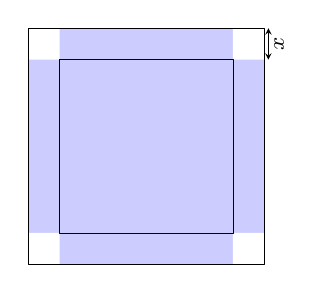
\begin{tikzpicture}[>=stealth,line join=round,line cap=round,font=\footnotesize,scale=1]
			\fill[blue!20] (0,0)--(3,0)--(3,3)--(0,3);
			\fill[white] (0,0)--(0,0.4)--(0.4,0.4)--(0.4,0) (2.6,0)--(3,0)--(3,0.4)--(2.6,0.4)
			(2.6,2.6)--(2.6,3)--(3,3)--(3,2.6) (0,2.6)--(0.4,2.6)--(0.4,3)--(0,3);
			\draw (0,0)--(3,0)--(3,3)--(0,3)--cycle;
			\draw[line width=0.2pt] (0.4,0.4)--(2.6,0.4)--(2.6,2.6)--(0.4,2.6)--cycle;
			\draw [line width=0.05pt,<->] (3.05,2.6)--(3.05,3);
			\path (3,2.6)--(3,3)node[pos=0.5,sloped,black,below]{$x$};					
		\end{tikzpicture}~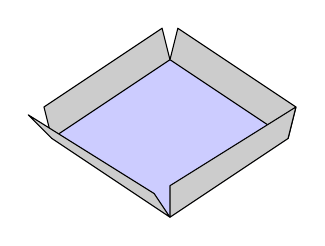
\begin{tikzpicture}[>=stealth,line join=round,line cap=round,font=\footnotesize,scale=1]
			\fill[blue!20] (0,0)--(1.5,-1)--(3,0)--(1.5,1);		
			\fill[black!20] (0,0)--(-0.1,0.4)--(1.4,1.4)--(1.5,1);
			\draw (0,0)--(-0.1,0.4)--(1.4,1.4)--(1.5,1)--cycle;
			\fill[black!20] (1.5,1)--(1.6,1.4)--(3.1,0.4)--(3,0);
			\draw (1.5,1)--(1.6,1.4)--(3.1,0.4)--(3,0)--cycle;
			\fill[black!20] (1.5,-1)--(1.5,-0.6)--(3.1,0.4)--(3,0);
			\draw (1.5,-1)--(1.5,-0.6)--(3.1,0.4)--(3,0)--cycle;
			\fill[black!20] (1.5,-1)--(1.3,-0.7)--(-0.3,0.3)--(0,0);
			\draw (1.5,-1)--(1.3,-0.7)--(-0.3,0.3)--(0,0)--cycle;
		\end{tikzpicture}
	\end{center}
	
	Bạn Việt muốn tìm độ dài cạnh hình vuông cần cắt bỏ để chiếc hộp đạt thể tích lớn nhất.
	\begin{enumerate}
		\item Hãy thiết lập hàm số biểu thị thể tích hộp theo $x$ với $x$ là độ dài cạnh hình vuông cần cắt đi.
		\item Khảo sát và vẽ đồ thị hàm số tìm được.\\		
		Từ đó, hãy tư vấn cho bạn Việt cách giải quyết vấn đề và giải thích vì sao cần chọn giá trị này. (Làm tròn kết quả đến hàng phần mười.)
	\end{enumerate}
	\loigiai{
		\begin{enumerate}
			\item Hãy thiết lập hàm số biểu thị thể tích hộp theo $x$ với $x$ là độ dài cạnh hình vuông cần cắt đi.
			Mặt đáy của hộp là hình vuông có cạnh bằng $6-2x$ (cm), với $0<x<3$. Vậy diện tích của đáy hộp là $S=(6-2x)^2$.\\
			Khối hộp có chiều cao $h=x$ (cm).\\
			Vậy thể tích hộp là $V=S\cdot h=(6-2x)^2 \cdot x=4x^3-24x^2+36x$ (cm$^3$).
			\item Khảo sát và vẽ đồ thị hàm số tìm được.\\
			Xét hàm $f(x)=4x^3-24x^2+36x,\,\,0<x<3$.
			\begin{enumerate}
				\item Tập xác định: $\mathscr{D}=(0;3)$.
				\item Sự biến thiên.
				\begin{itemize}
					\item Giới hạn tại vô cực: $\displaystyle\displaystyle\lim \limits{n \to +\infty}_{x \rightarrow+\infty} f(x)=+\infty, \displaystyle\displaystyle\lim \limits{n \to +\infty}_{x \rightarrow-\infty} f(x)=-\infty$.
					\item Ta có $f'(x)=12x^2-48x+36\Rightarrow f'(x)=0\Leftrightarrow x^2-4x+3=0\Leftrightarrow \hoac{& x=1\\ & x=3.}$\\
					Ta có bảng biến thiên:
					\begin{center}
						
\begin{tikzpicture}[>=stealth]
							\tkzTabInit[nocadre=false,lgt=1,espcl=2,deltacl=0.5]{$x$/.7 ,$y'$/.7,$y$/2}
							{$0$, $1$ , $3$ }
							\tkzTabLine{ , + , $0$ , - , $0$ }
							\tkzTabVar{-/$0$ , +/$16$ , -/$0$ }
						\end{tikzpicture}
					\end{center}
					Hàm số đồng biến trên $(0;1)$ và nghịch biến trên khoảng $(1;3)$.\\
					Hàm số không có cực trị.
					\item Đồ thị hàm số đi qua các điểm $(0 ; 0),(1 ; 16),(3 ; 0)$.
					\begin{center}
						\begin{tikzpicture}[line cap=butt,line join=miter,>=stealth,scale=0.8,font=\footnotesize,y=0.5cm]
							\tikzset{declare function={xmin=-1;xmax=4;ymin=-1;ymax=17;},
								smooth,samples=450}
							\draw[->] (xmin,0)--(xmax,0) node[shift={(0:7pt)},]{$ x $};
							\draw[->] (0,ymin)--(0,ymax) node[shift={(90:7pt)}]{$ y $};
							\fill (0,0) node[shift={(-150:7pt)}]{$ O $};
							\clip (xmin,ymin) rectangle (xmax,ymax);
							\foreach \i in {1}{
								\draw(\i,1.5pt)--(\i,-1.5pt)node[below]{$\i$};}
							\foreach \j in {16}{
								\draw(-1.5pt,\j)--(1.5pt,\j) node[left]{$\j$};}
							%	\draw(-1.5pt,-1)--(1.5pt,-1)node[shift={(7pt,0pt)}]{$-1$};	
							\def\f(#1){4*(#1)^3-24*(#1)^2+36*(#1)} % Đồ thị hàm số y=x^3+3x^2+3x+1
							\def\c{-1}
							\def\d{0}
							\def\e{-2}	
							\pgfmathsetmacro\fc{\f(\c)}
							\pgfmathsetmacro\fd{\f(\d)}
							\pgfmathsetmacro\fe{\f(\e)}
							\draw[samples=100] plot[domain=0:3] (\x,{\f(\x)});
							\foreach \x/\y in {\c/\fc,\d/\fd,\e/\fe}{
								\draw[dashed] (1,0)--(1,16)--(0,16);
								\fill[white,draw=black] (\x,\y) circle (1pt);}	
							%\node at (-2,-3.2) [right,fill=white,font=\footnotesize]{\it Hình LT $2b$};
						\end{tikzpicture}
					\end{center}
				\end{itemize}
			\end{enumerate}
			Vậy hình vuông mà bạn Việt cần cắt bỏ pải có độ dài cạnh $x=1$ dm thì chiếc hộp đạt thể tích lớn nhất.
		\end{enumerate}
	}
\end{bt}
